\chapter{Servicio de mensajería: privado y anónimo}

El trabajo sobre el cual se basa esta memoria consiste en el desarrollo de un sistema de mensajería que implemente funcionalidades que protejan tanto la identidad como la privacidad de sus usuarios. Para ello, la intención ha sido mezclar las dos tecnologías estado del arte en ambos panoramas, el protocolo Signal y el protocolo TOR. \\

El servidor se ha desarrollado en Node.js, haciendo uso de la librería para el manejo de websockets Socket.io. \\

Por otro lado, el cliente de escritorio hace uso de la librería Electron, de la cual se obtiene una base para un desarrollo sencillo multiplataforma. Se ha hecho uso también del framework React junto con Redux, para implementar la lógica de la vista de usuario y manejar las conexiones. \\

Además, se ha implementado a modo de experimento una versión del sistema para la mensajería en dispositivos móviles, aunque este carece de la funcionalidad de cifrado y ofuscación de identidad. Para este fin se ha hecho uso de la tecnología React Native. \\

El protocolo Signal se ha implementado mediante el uso de la librería creada por la organización Open Whispers Systems para el desarrollo de proyectos en Javascript. \\

En cuanto a la inclusión de TOR en la comunicación de la plataforma, se ha creado un hidden service (servicio en la red TOR), y se ha trabajado de cara a la conexión a través de esta red. Un requerimiento para conseguir tal conexión es entablar comunicación mediante el protocolo SOCKS, para el cual no existe actualmente adaptación por parte de la librería de websockets utilizada. A pesar de invertir una cantidad considerable de tiempo y esfuerzo en su inclusión, no ha sido posible implementar la comunicación a través de dicha red. Queda pues como una característica a implementar en el futuro, en la que se trabajará fuera del marco del trabajo de fin de grado. \\ 

A continuación se han añadido capturas de pantalla del uso de la aplicación: \\

\begin{figure}[H]
	\centering
	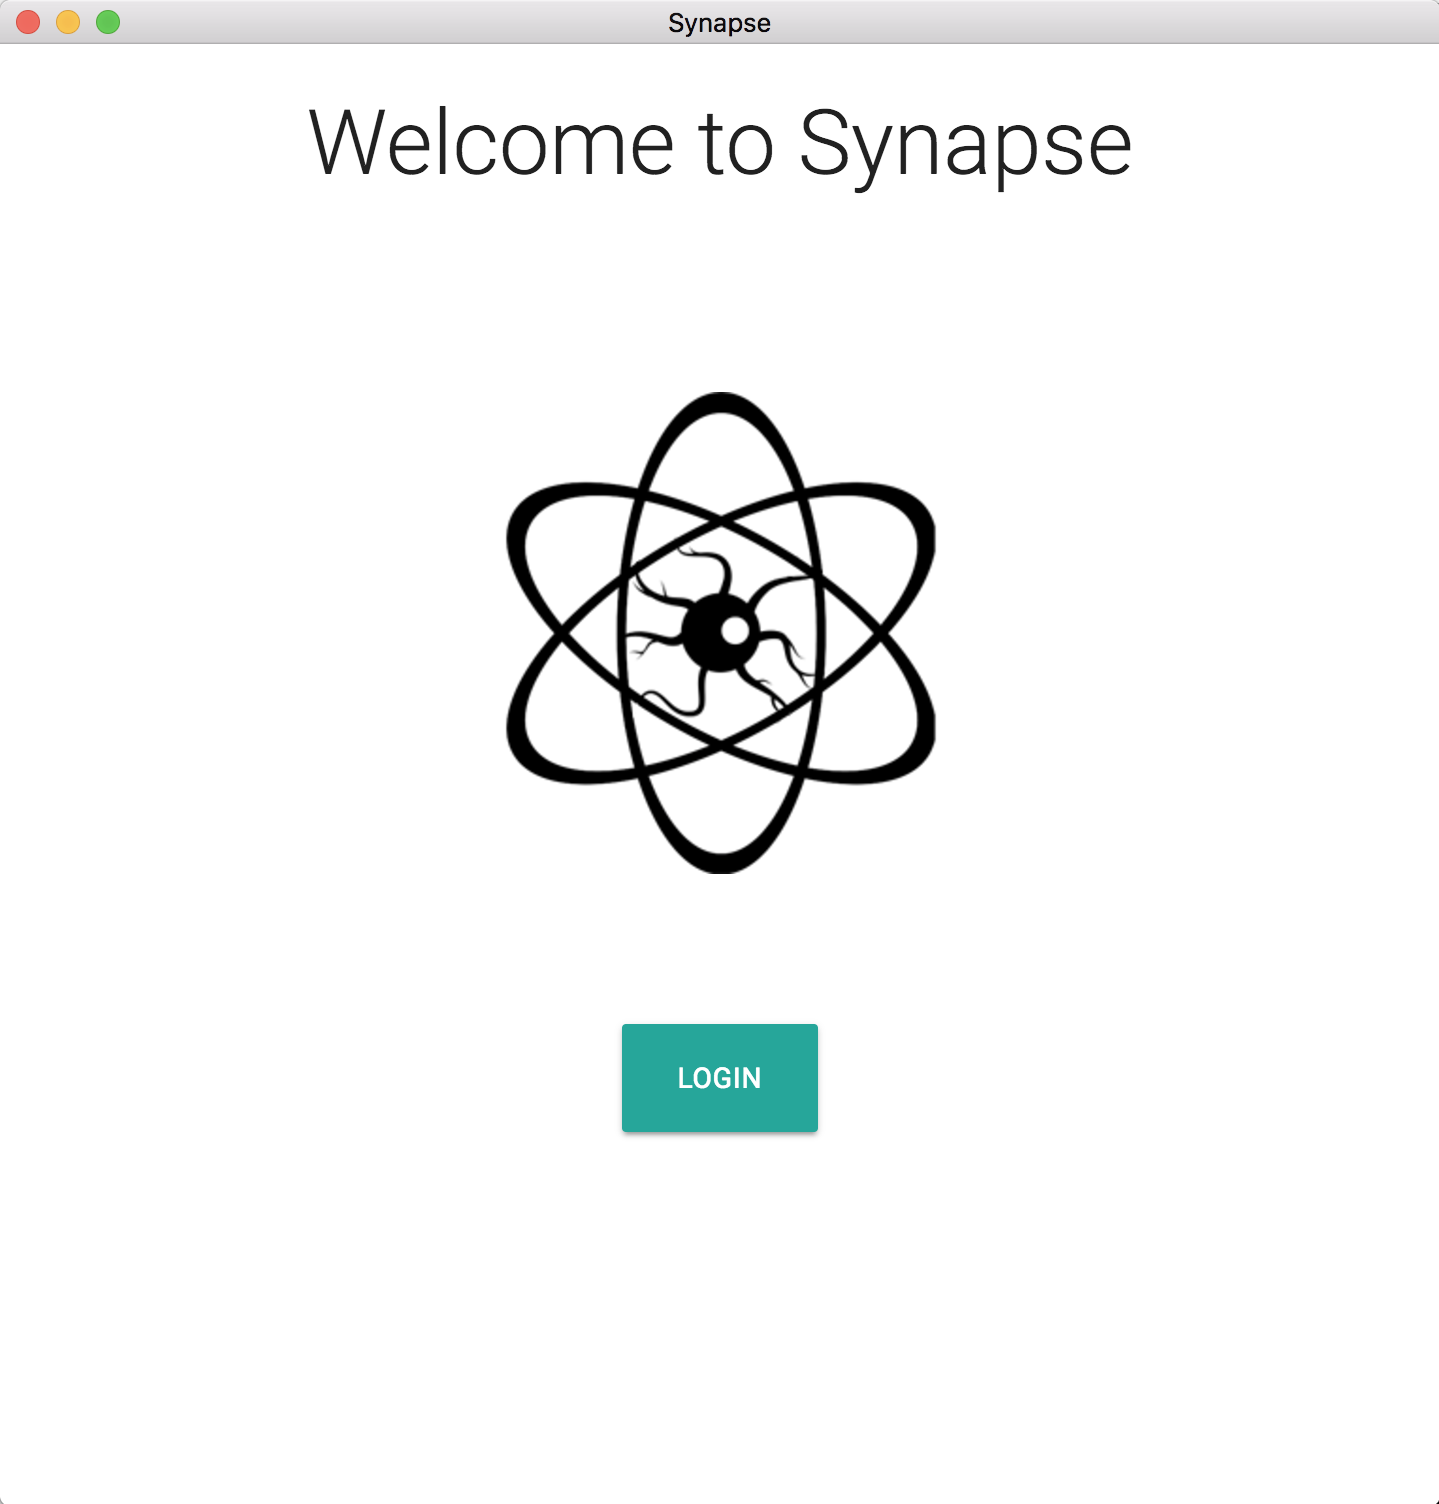
\includegraphics[width=\textwidth]{imagenes/desktop-landing-page}
	\caption{Página inicial}
	\label{fig:desktop-landing-page}
\end{figure}

\begin{figure}[H]
	\centering
	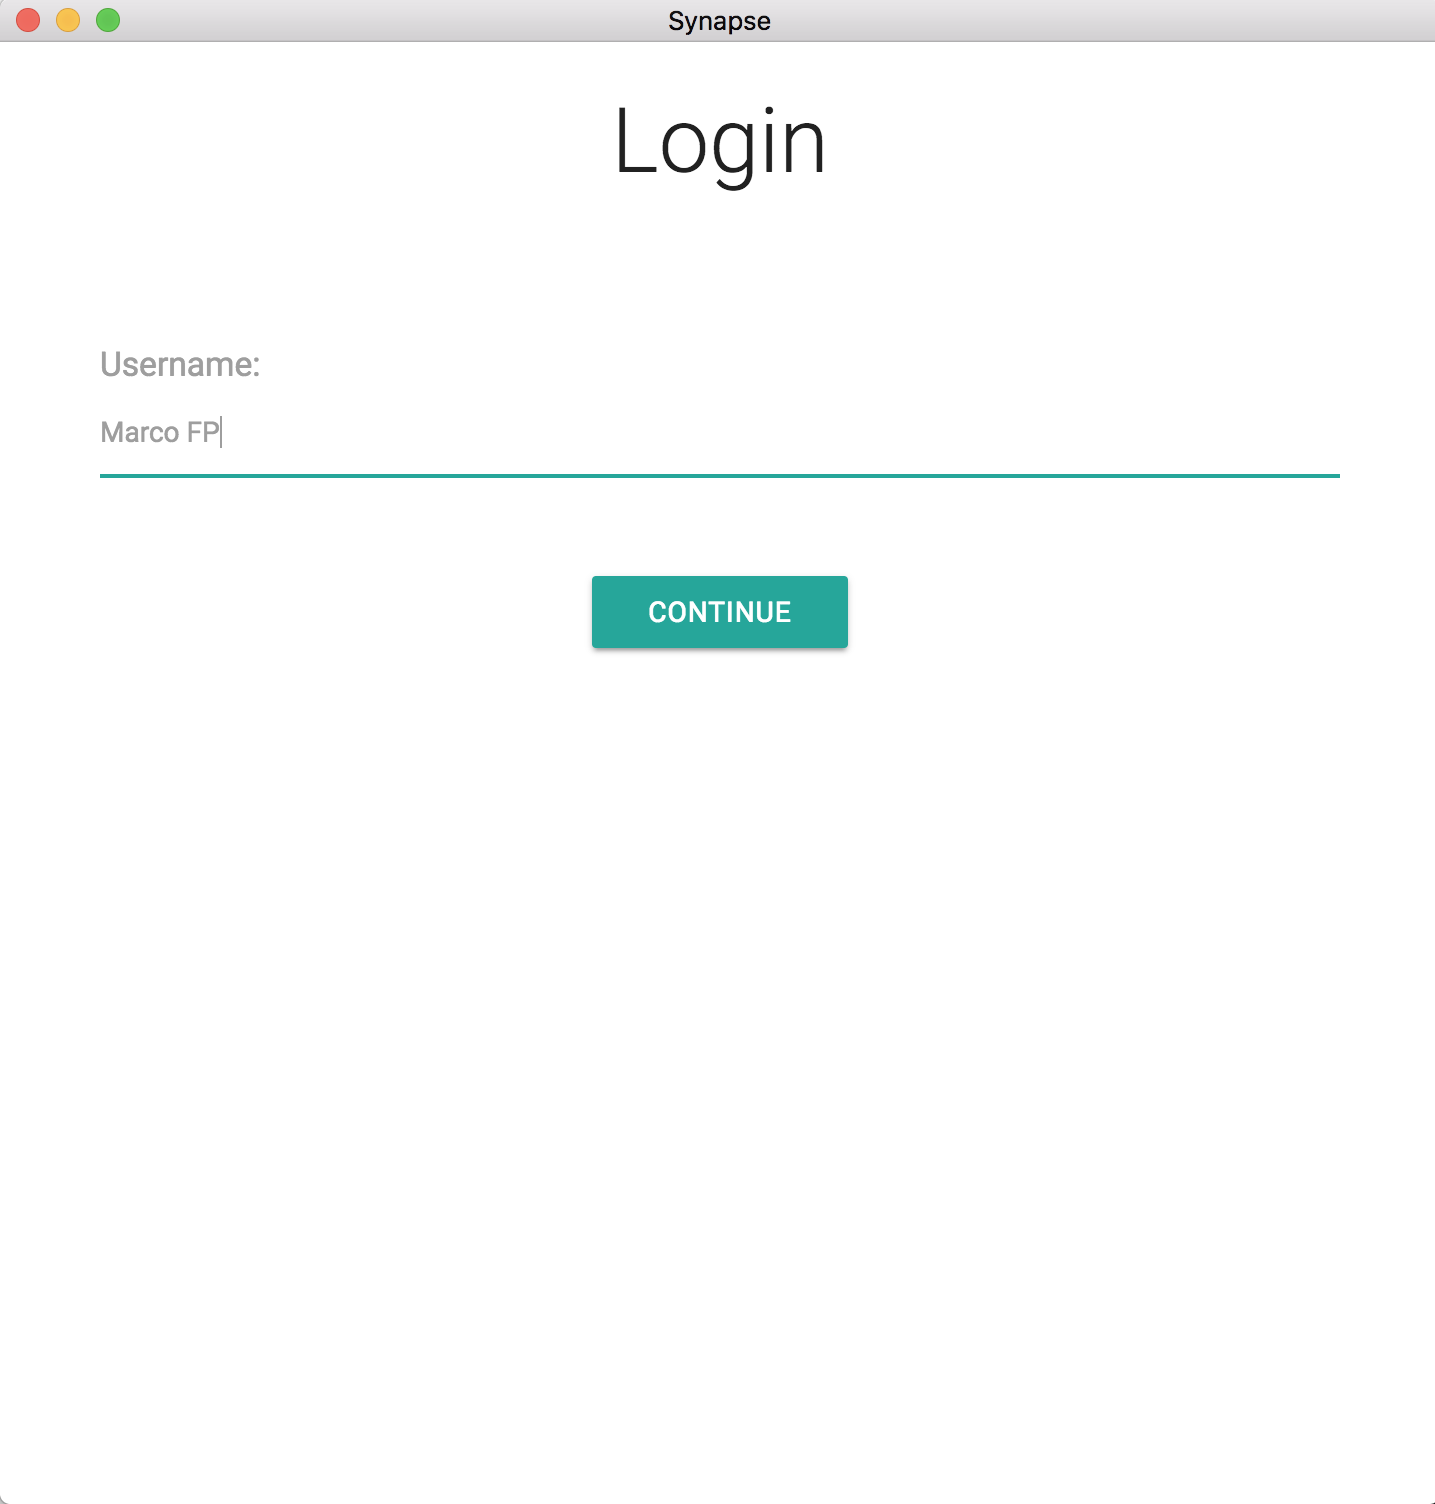
\includegraphics[width=\textwidth]{imagenes/desktop-login-page}
	\caption{Página de inicio de sesión y registro}
	\label{fig:desktop-login}
\end{figure}

\begin{figure}[H]
	\centering
	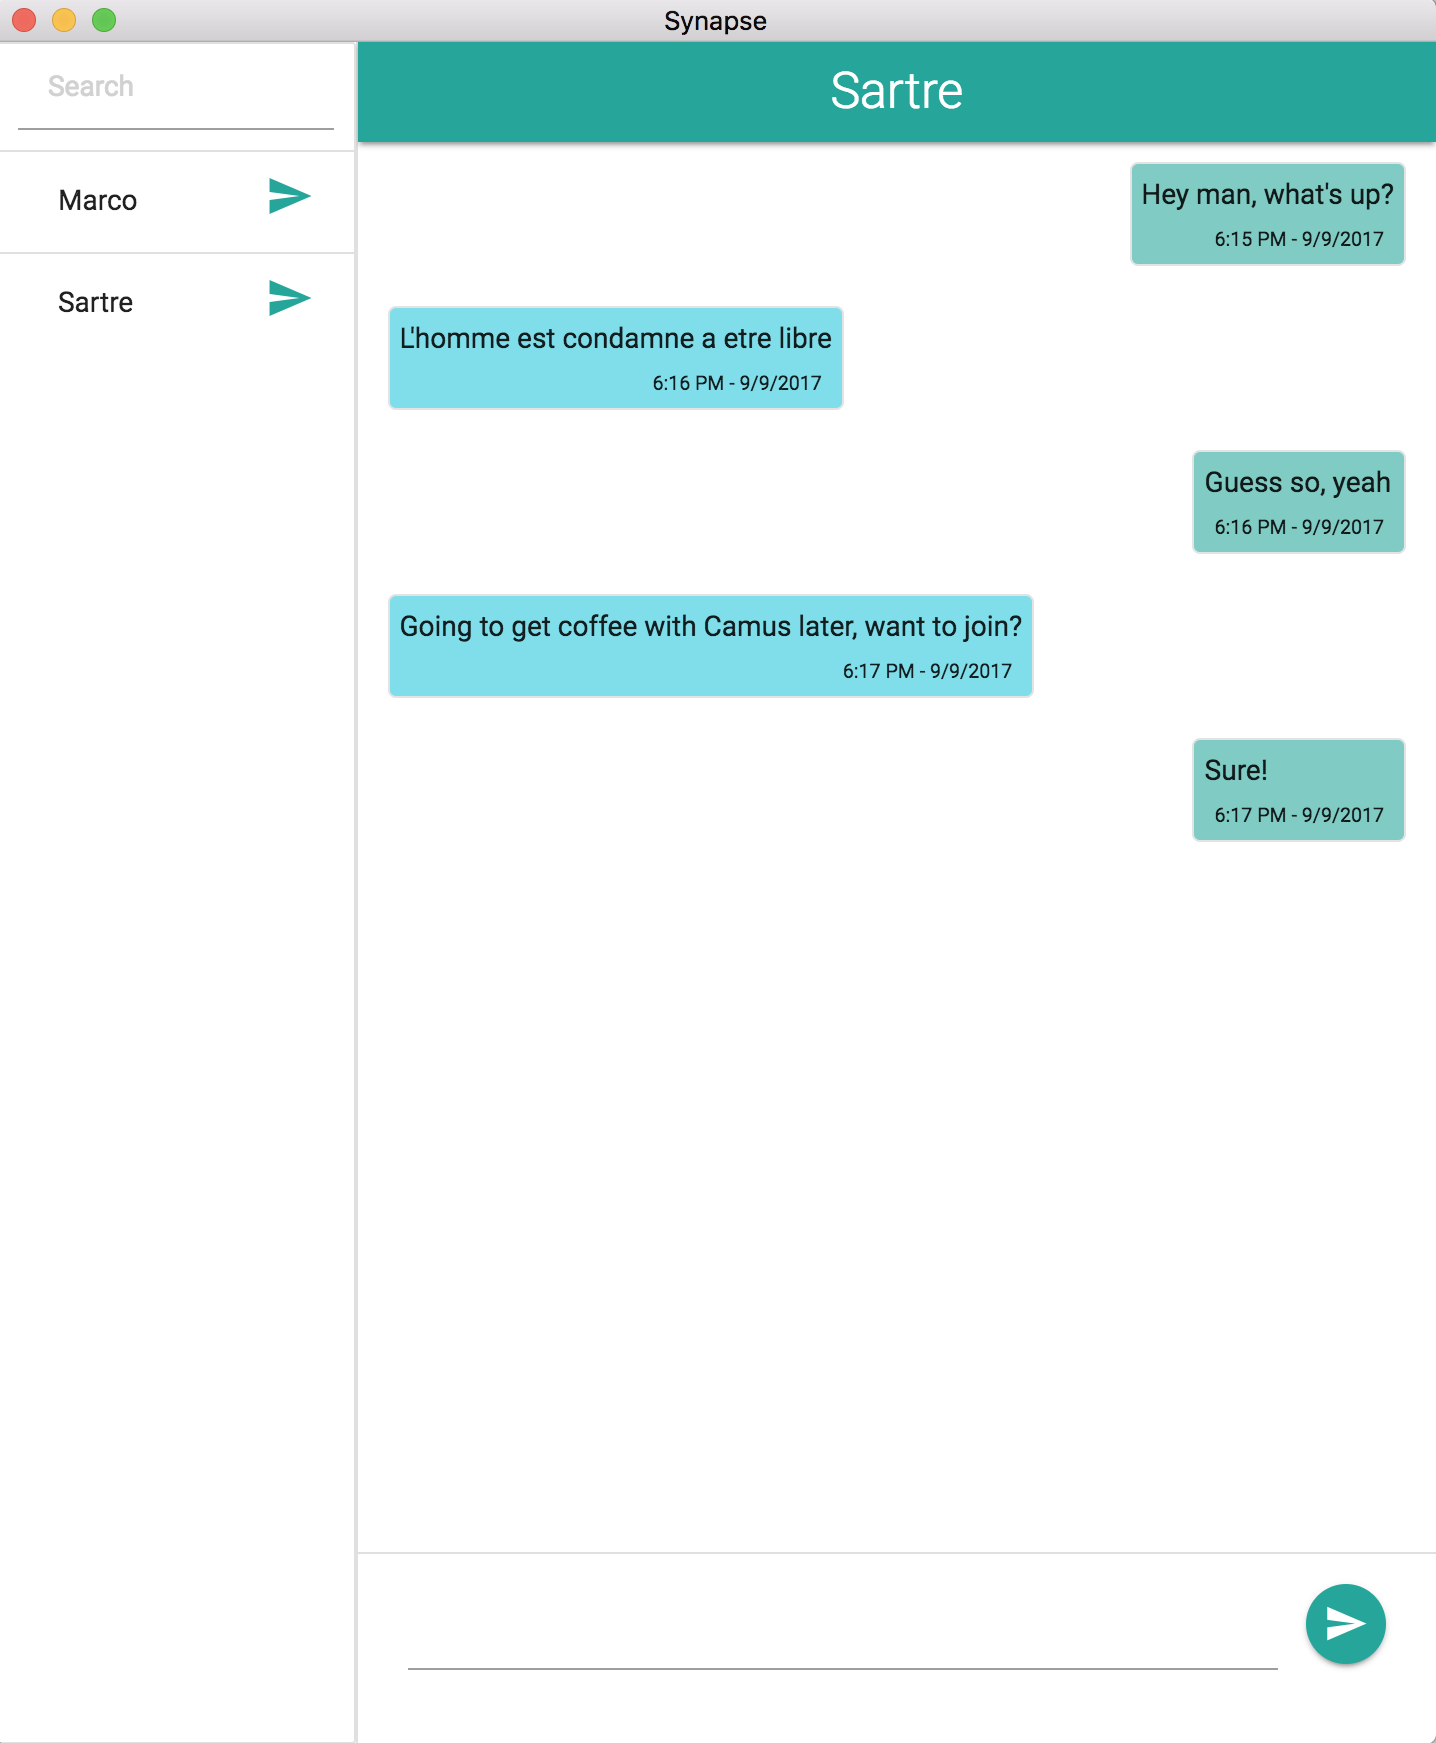
\includegraphics[width=\textwidth]{imagenes/desktop-conversation-page}
	\caption{Página de conversación}
	\label{fig:desktop-conversation}
\end{figure}